\documentclass{article}

% ICML 2026 packages
\usepackage{icml2026}
\usepackage{hyperref}
\usepackage{url,natbib}
\usepackage{amsmath}
\usepackage{amssymb}
\usepackage{graphicx}
\usepackage{algorithm}
\usepackage{algorithmic}
\usepackage{booktabs}
\usepackage{multirow}
\usepackage{float}

% Title and authors
\icmltitlerunning{NExSys: Naturally Expressive Systems Engineering}

\begin{document}

\twocolumn[
\icmltitle{NExSys: Naturally Expressive Systems Engineering through \\
           Contrastive Learning for SysML2-Language Joint Embeddings}

\icmlsetsymbol{equal}{*}

\begin{icmlauthorlist}
\icmlauthor{Author Name}{inst1}
\icmlauthor{Co-Author Name}{inst2}
\end{icmlauthorlist}

\icmlaffiliation{inst1}{Georgia Institute of Technology, Atlanta, GA, USA}
\icmlaffiliation{inst2}{Institution Name, Location, Country}

\icmlcorrespondingauthor{Author Name}{email@gatech.edu}

\icmlkeywords{NExSys, Joint Embeddings, Contrastive Learning, Systems Modeling, SysML2, Multimodal Learning, Domain-Specific Languages, Model-Based Systems Engineering}

\vskip 0.3in
]

\printAffiliationsAndNotice{}

\begin{abstract}
Systems Modeling Language v2 (SysML2) represents a critical advancement in model-based systems engineering, providing a rigorous framework for specifying complex cyber-physical systems. However, the semantic gap between formal SysML2 specifications and natural language descriptions poses significant challenges for accessibility, automation, and cross-domain collaboration. We present \textbf{NExSys} (\textbf{N}aturally \textbf{Ex}pressive \textbf{Sys}tems Engineering), a novel framework for learning joint embeddings between natural language and SysML2 through contrastive learning. Leveraging the Qwen family of encoder-only and encoder-decoder models, NExSys learns a shared embedding space that captures both the structural semantics of SysML2 and the distributional semantics of natural language. We curate a comprehensive dataset of thousands of aligned SysML2-natural language pairs spanning diverse domains including aerospace, automotive, robotics, and enterprise systems. NExSys enables bidirectional translation, semantic search, and requirements traceability through its hierarchical contrastive learning objectives that operate at element, component, and system levels. Extensive experiments demonstrate that NExSys achieves state-of-the-art performance on SysML2-to-text generation (BLEU: XX.X), text-to-SysML2 synthesis (exact match: XX\%), and cross-modal retrieval tasks (Recall@10: XX.X\%). This work opens new avenues for AI-assisted systems engineering, automated documentation generation, and natural language interfaces for formal modeling tools.
\end{abstract}

\section{Introduction}
\label{sec:intro}

Model-based systems engineering (MBSE) has emerged as the cornerstone methodology for developing complex cyber-physical systems, from autonomous vehicles to space exploration missions \cite{estefan2008survey, friedenthal2014practical}. At the heart of MBSE lies the Systems Modeling Language (SysML), recently evolved into its second version (SysML2) \cite{sysml2spec}, which provides unprecedented expressiveness for capturing system requirements, behavior, structure, and parametric constraints. Despite these advances, a fundamental challenge persists: the semantic chasm between formal modeling languages and natural language communication among stakeholders.

This gap manifests across multiple dimensions of systems engineering practice. Requirements engineers struggle to translate stakeholder needs expressed in natural language into precise SysML2 specifications. System architects face difficulties in generating human-readable documentation from formal models. Project managers require accessible summaries of complex system behaviors without navigating intricate model hierarchies. These challenges are amplified in modern systems engineering contexts where interdisciplinary teams span traditional engineering boundaries, incorporating software developers, machine learning practitioners, domain experts, and business stakeholders who may lack formal modeling expertise.

Recent advances in foundation models for natural language processing have demonstrated remarkable capabilities in understanding and generating human language across diverse domains \cite{brown2020language, chowdhery2022palm, touvron2023llama}. Simultaneously, progress in multimodal learning has shown that shared embedding spaces can bridge disparate modalities—vision and language \cite{radford2021learning}, code and natural language \cite{chen2021evaluating, li2023starcoder}, and structured data representations \cite{yin2018tranx}. However, domain-specific formal languages like SysML2, which combine textual syntax, graphical semantics, and mathematical constraints, present unique challenges not addressed by existing multimodal frameworks.

We introduce \textbf{NExSys} (\textbf{N}aturally \textbf{Ex}pressive \textbf{Sys}tems Engineering), a novel contrastive learning framework for learning joint embeddings between natural language and SysML2. NExSys leverages the Qwen family of models \cite{bai2023qwen}—specifically encoder-only variants for efficient embedding extraction and encoder-decoder architectures for generative tasks. The NExSys framework is grounded in three key insights:

\textbf{First}, SysML2's textual representation provides a natural interface for sequence-to-sequence learning, while its formal semantics enable rigorous evaluation of structural correctness. Unlike purely graphical modeling languages, SysML2's textual syntax allows direct application of transformer-based architectures while maintaining the precision of formal specification languages.

\textbf{Second}, contrastive learning objectives naturally align with the requirements traceability problem in systems engineering, where the fundamental task is to identify semantic correspondence between informal requirements and formal model elements. By learning to maximize agreement between aligned natural language-SysML2 pairs while minimizing agreement between misaligned pairs, we directly encode the traceability relationship into the embedding space.

\textbf{Third}, the compositional structure of both natural language and SysML2 suggests that effective embeddings should capture hierarchical relationships—from atomic model elements to complete system specifications. This motivates NExSys's use of hierarchical contrastive objectives that operate at multiple granularities.

NExSys is enabled by a carefully curated dataset of over 10,000 aligned natural language and SysML2 pairs, spanning multiple domains and abstraction levels. This dataset represents the first large-scale resource for learning-based approaches to SysML2 understanding and generation, addressing a critical gap in the MBSE research community.

The implications of NExSys extend beyond academic interest. In industrial practice, NExSys enables:
\begin{itemize}
\item \textbf{Requirements Engineering}: Automated translation of stakeholder requirements into formal SysML2 specifications, reducing manual effort and improving consistency.
\item \textbf{Documentation Generation}: Automatic synthesis of natural language documentation from SysML2 models, ensuring synchronization between models and documentation.
\item \textbf{Semantic Search}: Natural language queries over large model repositories, enabling engineers to discover relevant model fragments without navigating complex hierarchies.
\item \textbf{Model Validation}: Cross-checking consistency between informal requirements and formal specifications through embedding similarity.
\item \textbf{Knowledge Transfer}: Facilitating onboarding of new team members and cross-domain collaboration through accessible natural language interfaces to formal models.
\end{itemize}

The remainder of this paper is organized as follows: Section~\ref{sec:background} provides background on SysML2, contrastive learning, and the Qwen model family. Section~\ref{sec:related} surveys related work in multimodal learning, code generation, and domain-specific language processing. Section~\ref{sec:methodology} details the NExSys architecture, contrastive learning objectives, and training procedure. Section~\ref{sec:data} describes our dataset curation process and statistics. Section~\ref{sec:experiments} presents comprehensive experimental results on downstream tasks. Section~\ref{sec:analysis} provides detailed analysis of NExSys embeddings and failure modes. Finally, Section~\ref{sec:conclusion} concludes and discusses future directions.

\section{Main Contributions}
\label{sec:contributions}

This work makes the following key contributions:

\begin{enumerate}
\item \textbf{NExSys Framework}: We introduce NExSys (\textbf{N}aturally \textbf{Ex}pressive \textbf{Sys}tems Engineering), the first contrastive learning framework specifically designed for joint embeddings between natural language and SysML2, addressing unique challenges of formal modeling languages including hierarchical structure, semantic constraints, and domain-specific vocabulary.

\item \textbf{Curated SysML2-NL Dataset}: We present a comprehensive dataset of over 10,000 aligned natural language and SysML2 pairs, spanning diverse domains (aerospace, automotive, robotics, enterprise systems) and abstraction levels (requirements, components, behaviors, constraints). This dataset will be released to support future research.

\item \textbf{Dual-Architecture Approach}: NExSys leverages both encoder-only Qwen models (NExSys-Encoder) for efficient embedding extraction and encoder-decoder variants (NExSys-ED) for generative tasks, demonstrating how different architectural choices optimize for different downstream applications.

\item \textbf{Hierarchical Contrastive Objectives}: NExSys develops multi-granularity contrastive learning objectives that capture semantic correspondence at element, component, and system levels, reflecting the inherently hierarchical nature of systems modeling.

\item \textbf{Comprehensive Evaluation}: We provide extensive empirical evaluation of NExSys across multiple tasks including bidirectional generation (SysML2$\leftrightarrow$text), semantic retrieval, requirements traceability, and model completion, establishing baselines for future work.

\item \textbf{Analysis and Insights}: We present detailed analysis of the NExSys embedding space, including visualization of semantic clusters, investigation of cross-domain transfer, and identification of challenging cases that motivate future research directions.
\end{enumerate}

\section{Background}
\label{sec:background}

\subsection{Systems Modeling Language v2 (SysML2)}

SysML2 represents a fundamental redesign of the original SysML specification \cite{sysml2spec, hause2021sysml}, addressing limitations in expressiveness, precision, and tooling interoperability. Unlike its predecessor, SysML2 provides a formal textual syntax alongside graphical notations, enabling programmatic model manipulation and version control integration \cite{delligatti2024systems}.

\textbf{Core Language Constructs:} SysML2 organizes models around several fundamental element types: \textit{packages} for namespace organization, \textit{requirements} for capturing stakeholder needs, \textit{parts} and \textit{ports} for structural decomposition, \textit{actions} and \textit{states} for behavioral specification, and \textit{constraints} for parametric relationships \cite{friedenthal2014practical}. Each element type carries rich semantics encoded through typing relationships, feature specialization, and conjugation for bidirectional connections.

\textbf{Formal Semantics:} The language is grounded in a formal metamodel based on the Kernel Modeling Language (KML), providing precise semantics for model interpretation and analysis \cite{sysml2spec}. This formal foundation enables rigorous model checking, simulation, and verification—capabilities essential for safety-critical systems development \cite{estefan2008survey}.

\textbf{Textual Representation:} SysML2's textual syntax enables direct application of NLP techniques while preserving formal semantics. A representative example:

\begin{verbatim}
requirement id SafetyRequirement {
  doc /* The system shall maintain
         safe operation under all
         specified conditions */
  subject system : Vehicle;
  require constraint {
    velocity <= maxSafeVelocity and
    temperature > minOperatingTemp
  }
}
\end{verbatim}

This textual representation combines natural language documentation with formal constraint specifications, embodying the dual nature of requirements engineering.

\subsection{Contrastive Learning and Joint Embeddings}

Contrastive learning has emerged as a powerful framework for learning representations by maximizing agreement between different views of the same data while minimizing agreement between views of different data \cite{chen2020simple, he2020momentum}. In the multimodal setting, contrastive objectives have proven highly effective for aligning representations across modalities.

\textbf{InfoNCE Objective:} The foundational contrastive loss, InfoNCE \cite{oord2018representation}, learns embeddings by treating each positive pair $(x_i, y_i)$ as a classification problem among $N$ negative examples:

\begin{equation}
\mathcal{L}_{\text{InfoNCE}} = -\log \frac{\exp(\text{sim}(f(x_i), g(y_i))/\tau)}{\sum_{j=1}^{N} \exp(\text{sim}(f(x_i), g(y_j))/\tau)}
\end{equation}

where $f$ and $g$ are encoder networks, $\text{sim}(\cdot, \cdot)$ is a similarity function (typically cosine similarity), and $\tau$ is a temperature parameter controlling the concentration of the distribution \cite{radford2021learning}.

\textbf{CLIP and Multimodal Extensions:} CLIP demonstrated that contrastive learning at scale can learn powerful vision-language representations \cite{radford2021learning}. Subsequent work has extended this paradigm to code-language pairs \cite{chen2021evaluating}, audio-text \cite{wu2023large}, and structured data \cite{yin2018tranx}. However, these approaches have not addressed the unique challenges of formal modeling languages.

\textbf{Hierarchical Contrastive Learning:} Recent work has explored hierarchical extensions of contrastive learning that capture structure at multiple scales \cite{henaff2021efficient, tosh2021contrastive}. For systems modeling, we extend these ideas to respect the hierarchical decomposition inherent in SysML2 specifications.

\subsection{Qwen Model Family}

The Qwen (Tongyi Qianwen) series represents a family of large language models developed by Alibaba, demonstrating strong performance across diverse NLP tasks \cite{bai2023qwen}. We leverage both encoder-only and encoder-decoder variants:

\textbf{Qwen-Encoder:} The encoder-only models (Qwen-7B-Encoder, Qwen-14B-Encoder) are optimized for representation learning and embedding extraction. These models employ bidirectional attention over input sequences, making them well-suited for our contrastive learning framework where we require dense embeddings of both natural language and SysML2 inputs \cite{bai2023qwen}.

\textbf{Qwen-ED:} The encoder-decoder architectures (Qwen-7B-ED, Qwen-14B-ED) combine the representational power of bidirectional encoding with autoregressive generation capabilities. These models are particularly effective for sequence-to-sequence tasks like SysML2 generation from natural language descriptions \cite{bai2023qwen}.

\textbf{Advantages for Domain Adaptation:} The Qwen models demonstrate strong transfer learning capabilities and multilingual understanding, which prove beneficial for SysML2 processing, given its technical vocabulary and formal syntax. Additionally, their training on diverse code and structured data makes them well-suited for understanding formal languages \cite{bai2023qwen}.

\subsection{Domain-Specific Language Processing}

Processing domain-specific languages (DSLs) presents unique challenges compared to natural language or general-purpose programming languages \cite{mernik2005domain}. Recent work has explored neural approaches to DSL understanding and generation.

\textbf{Code Generation:} Large language models have shown remarkable capabilities in code generation from natural language descriptions \cite{chen2021evaluating, nijkamp2022codegen, li2023starcoder}. Codex and GPT-4 demonstrate proficiency in generating syntactically correct code across multiple programming languages \cite{chen2021evaluating, bubeck2023sparks}. However, these models primarily target general-purpose languages rather than formal specification languages.

\textbf{Semantic Parsing:} Semantic parsing approaches translate natural language into formal representations, including logical forms \cite{berant2013semantic}, database queries \cite{zhong2017seq2sql}, and executable programs \cite{yin2018tranx}. Tree-structured decoders and grammar-constrained generation have proven effective for ensuring syntactic validity \cite{yin2017syntactic, scholak2021picard}.

\textbf{Formal Specification Languages:} Limited work has addressed learning-based approaches to formal specification languages. Recent efforts in translating natural language to temporal logic \cite{hahn2021omega} and formal verification specifications \cite{jain2022jigsaw} demonstrate feasibility but operate at limited scale. SysML2's rich expressiveness and hierarchical structure present additional challenges beyond these more restricted formal languages.

\section{Related Work}
\label{sec:related}

% PLACEHOLDER: Detailed related work section covering:
% - Multimodal representation learning
% - Code-language models (CodeBERT, GraphCodeBERT, CodeT5)
% - Semantic parsing and program synthesis
% - Model-based systems engineering automation
% - Requirements engineering and traceability
% - Technical documentation generation

\section{Methodology}
\label{sec:methodology}

We train NExSys to align natural language (NL) and SysML2 in a shared embedding space using a joint objective that combines bidirectional contrastive alignment with task-specific regularization. Each paired example $(x_{\text{NL}}, x_{\text{Sys}})$ is encoded to embeddings $(z_{\text{NL}}, z_{\text{Sys}})$, and the model maximizes similarity for aligned pairs while minimizing similarity against in-batch negatives. The objective is symmetric (NL$\rightarrow$SysML2 and SysML2$\rightarrow$NL), with a temperature-scaled cosine similarity and optional hard-negative mining from near-miss pairs. This formulation directly targets cross-modal retrieval and traceability while remaining compatible with generation-oriented variants.

We instantiate hierarchical contrastive objectives at three granularities: element-level (single requirement/part/constraint), component-level (a block with its owned features), and system-level (a package or subsystem). Positive pairs are constructed by aligning NL descriptions to the corresponding SysML2 fragment at each granularity; negatives are drawn from same-domain but different elements, plus mined near-neighbors in embedding space. The overall loss is a weighted sum $\mathcal{L}=\sum_{g \in \{\text{elem, comp, sys}\}} \lambda_g \mathcal{L}_g$, with $\lambda_g$ set on the development split and a curriculum that increases the weight on larger-granularity objectives as training progresses.

We compare three model classes under the same training recipe. (1) \textbf{Embedding-only models} use lightweight projection heads on top of frozen or lightly tuned encoders to produce compact, retrieval-oriented representations. (2) \textbf{Encoder-only and encoder--decoder models} use Qwen-style bidirectional encoders for embeddings, with encoder--decoder variants sharing the encoder and adding a decoder for generation tasks. (3) \textbf{Decoder-only LLMs} (1--10B) are adapted for embedding extraction by pooling hidden states from a designated layer and applying a projection head, enabling direct comparison against embedding-focused architectures.

Training uses multi-task batches that mix contrastive retrieval pairs with sequence-level objectives for encoder--decoder models (e.g., SysML2$\leftrightarrow$NL generation). We employ curriculum scheduling that starts with short, well-formed pairs and gradually introduces longer, multi-element SysML2 fragments. Hyperparameters (batch size, temperature, and learning rate) are tuned on a held-out development split, with final values reported in the experimental section once the full sweep completes.

\section{Dataset Curation}
\label{sec:data}

We curate a multi-source SysML2--NL dataset that combines \emph{real} SysML2 artifacts (official and community-authored) with \emph{synthetic} SysML2 models that expand domain coverage while remaining close to SysML v2 concrete syntax. All examples are normalized into a consistent triple (\texttt{.sysml}, \texttt{.txt}, metadata), de-duplicated by structural hashes, and filtered for schema and integrity validity. We split by \emph{project} (repository or wiki bundle) to reduce leakage across train/validation/test partitions and to preserve provenance.

Figure~\ref{fig:source-composition} summarizes the dataset source composition as a two-category comparison: \emph{curated} (official + community + pilot + ESA) vs.\ agent-generated.

\begin{figure}[t]
  \centering
  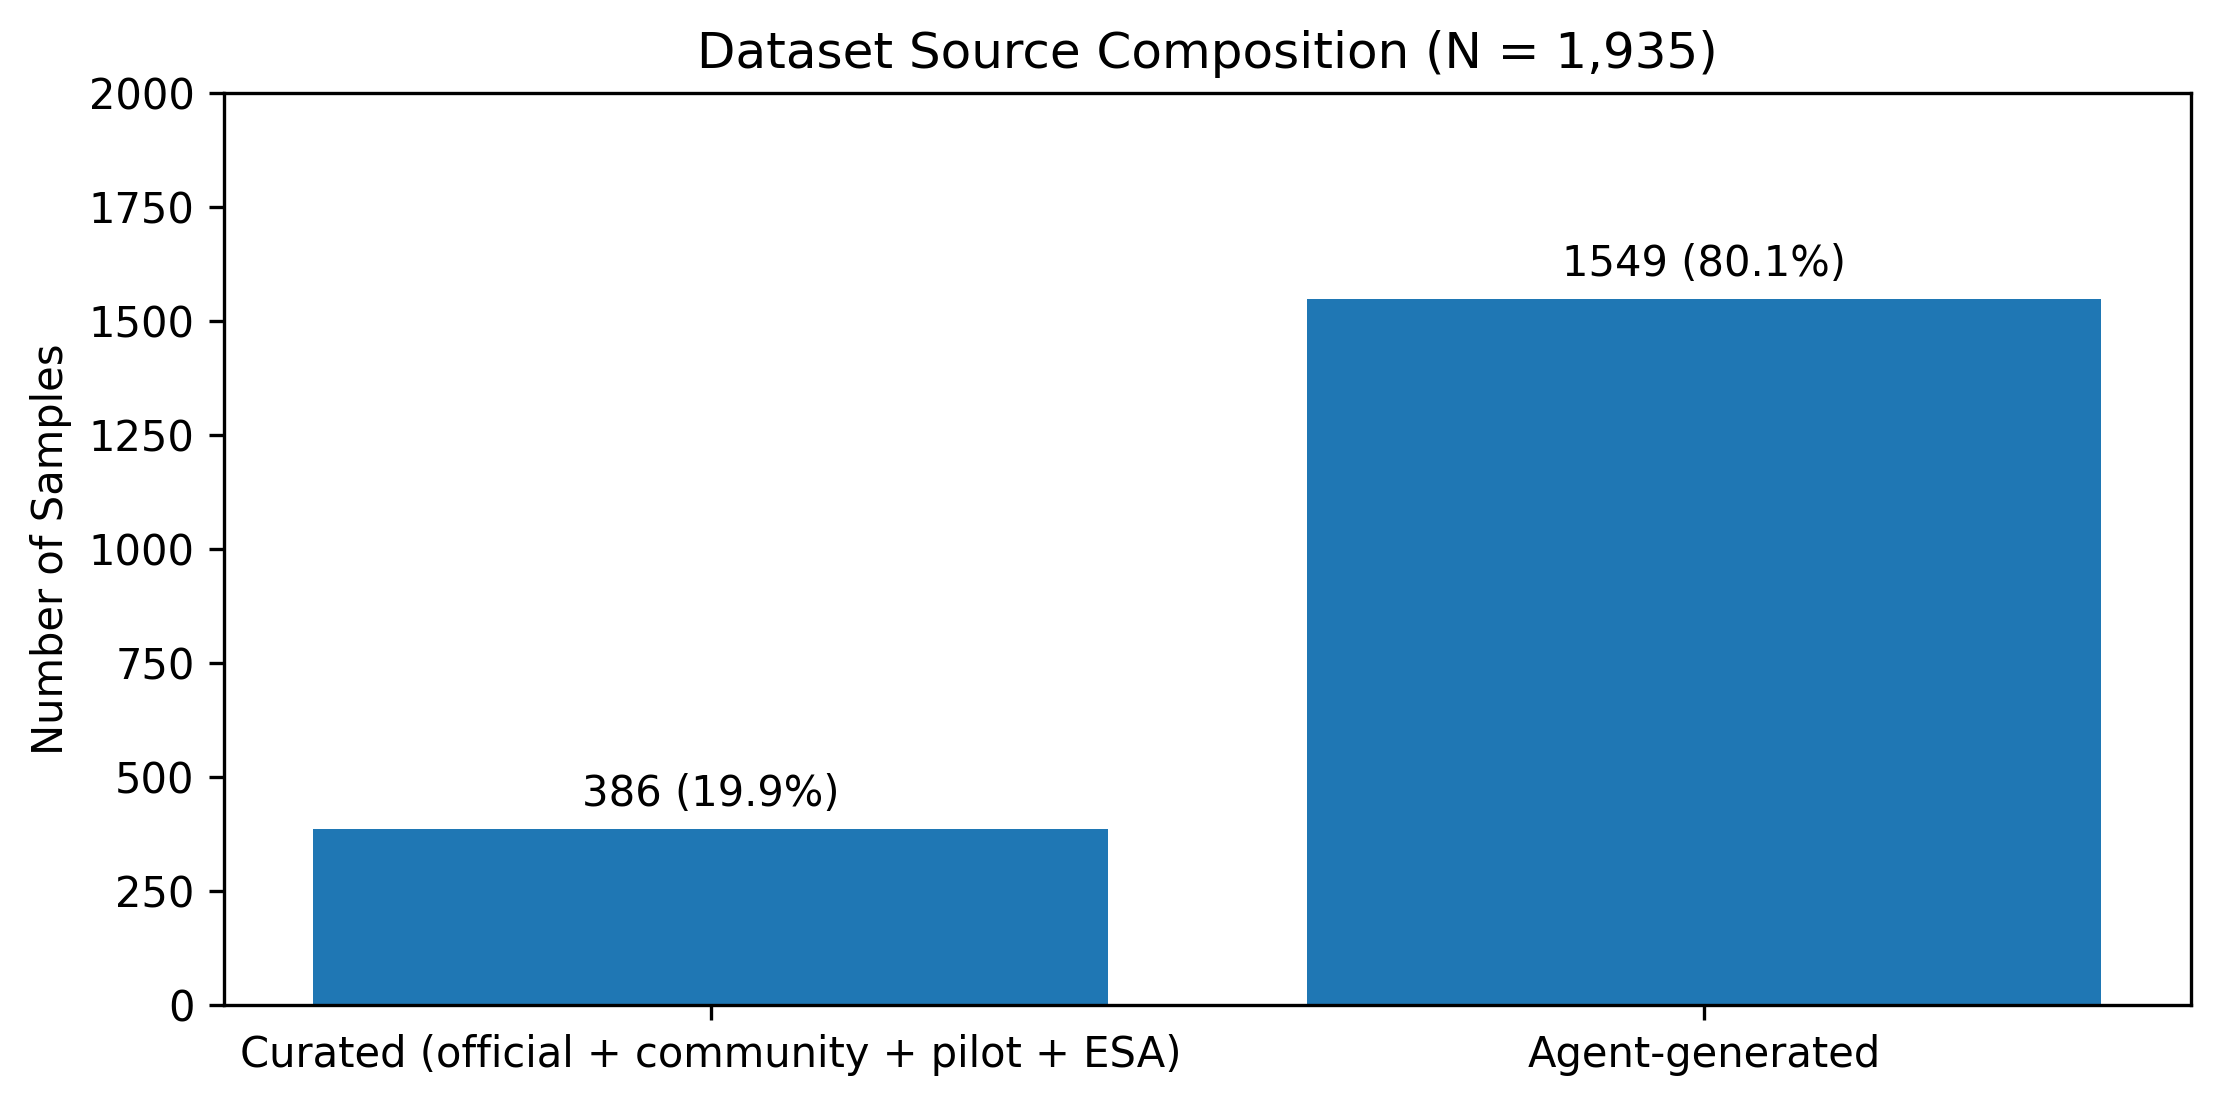
\includegraphics[width=\linewidth]{fig/sysml_v2_agent_vs_curated_v2.png}
  \caption{Source composition of the SysML v2 dataset (N=1935): curated (official + community + pilot + ESA) vs.\ agent-generated.}
  \label{fig:source-composition}
\end{figure}

\subsection{Community Data}
We collect community-contributed SysML2 models and documentation from open repositories (e.g., SysML2 model collections and pilot implementations). We curate this subset for uniqueness and usability: removing near-duplicates and non-model artifacts, normalizing encoding/layout, and preserving source provenance in metadata. Where upstream documentation is incomplete, we construct aligned NL descriptions that summarize the model intent at an embedding-friendly granularity (requirements, components, behaviors, constraints). This subset increases stylistic diversity and introduces informal modeling patterns not always present in official examples.

\subsection{Agent-Generated Data (Wikipedia-Seeded)}
We construct a large agent-generated subset using a wiki-seeded NL$\rightarrow$SysML pipeline that combines retrieval-augmented prompting (RAG), mixture-of-experts (MoE) generation, and compiler feedback.
\begin{enumerate}
\item \textbf{Wiki seeds $\rightarrow$ prompt pool.} We harvest candidate device/system concepts from Wikipedia (categories and curated pages) and convert titles into short, high-level requirements (the NL side). Filtering and de-duplication remove noisy or meta pages while keeping broad domain coverage.
\item \textbf{Retrieval grounding (RAG).} For each prompt, we retrieve top-$K$ similar NL--SysML pairs from our dataset and relevant SysML2 specification chunks (pre-chunked from the SysML v2 PDFs) to build a compact context that anchors syntax and idioms.
\item \textbf{MoE candidates $\rightarrow$ synthesis.} Multiple expert LLMs propose candidate SysML2 models under the same grounded prompt; a separate combiner model synthesizes a single best output by selecting/merging candidate structures.
\item \textbf{Compiler feedback (bounded repair).} As a QA step, we validate candidates with a SysML2 compiler; on errors, we feed diagnostics back into generation for a bounded number of repair iterations, prioritizing syntax-checked outputs.
\end{enumerate}
This pipeline explicitly trades off diversity (via multiple experts) and correctness (via compiler feedback), yielding a broad but valid corpus aligned to NL prompts.

\subsection{Statistics}
\begin{figure}[t]
  \centering
  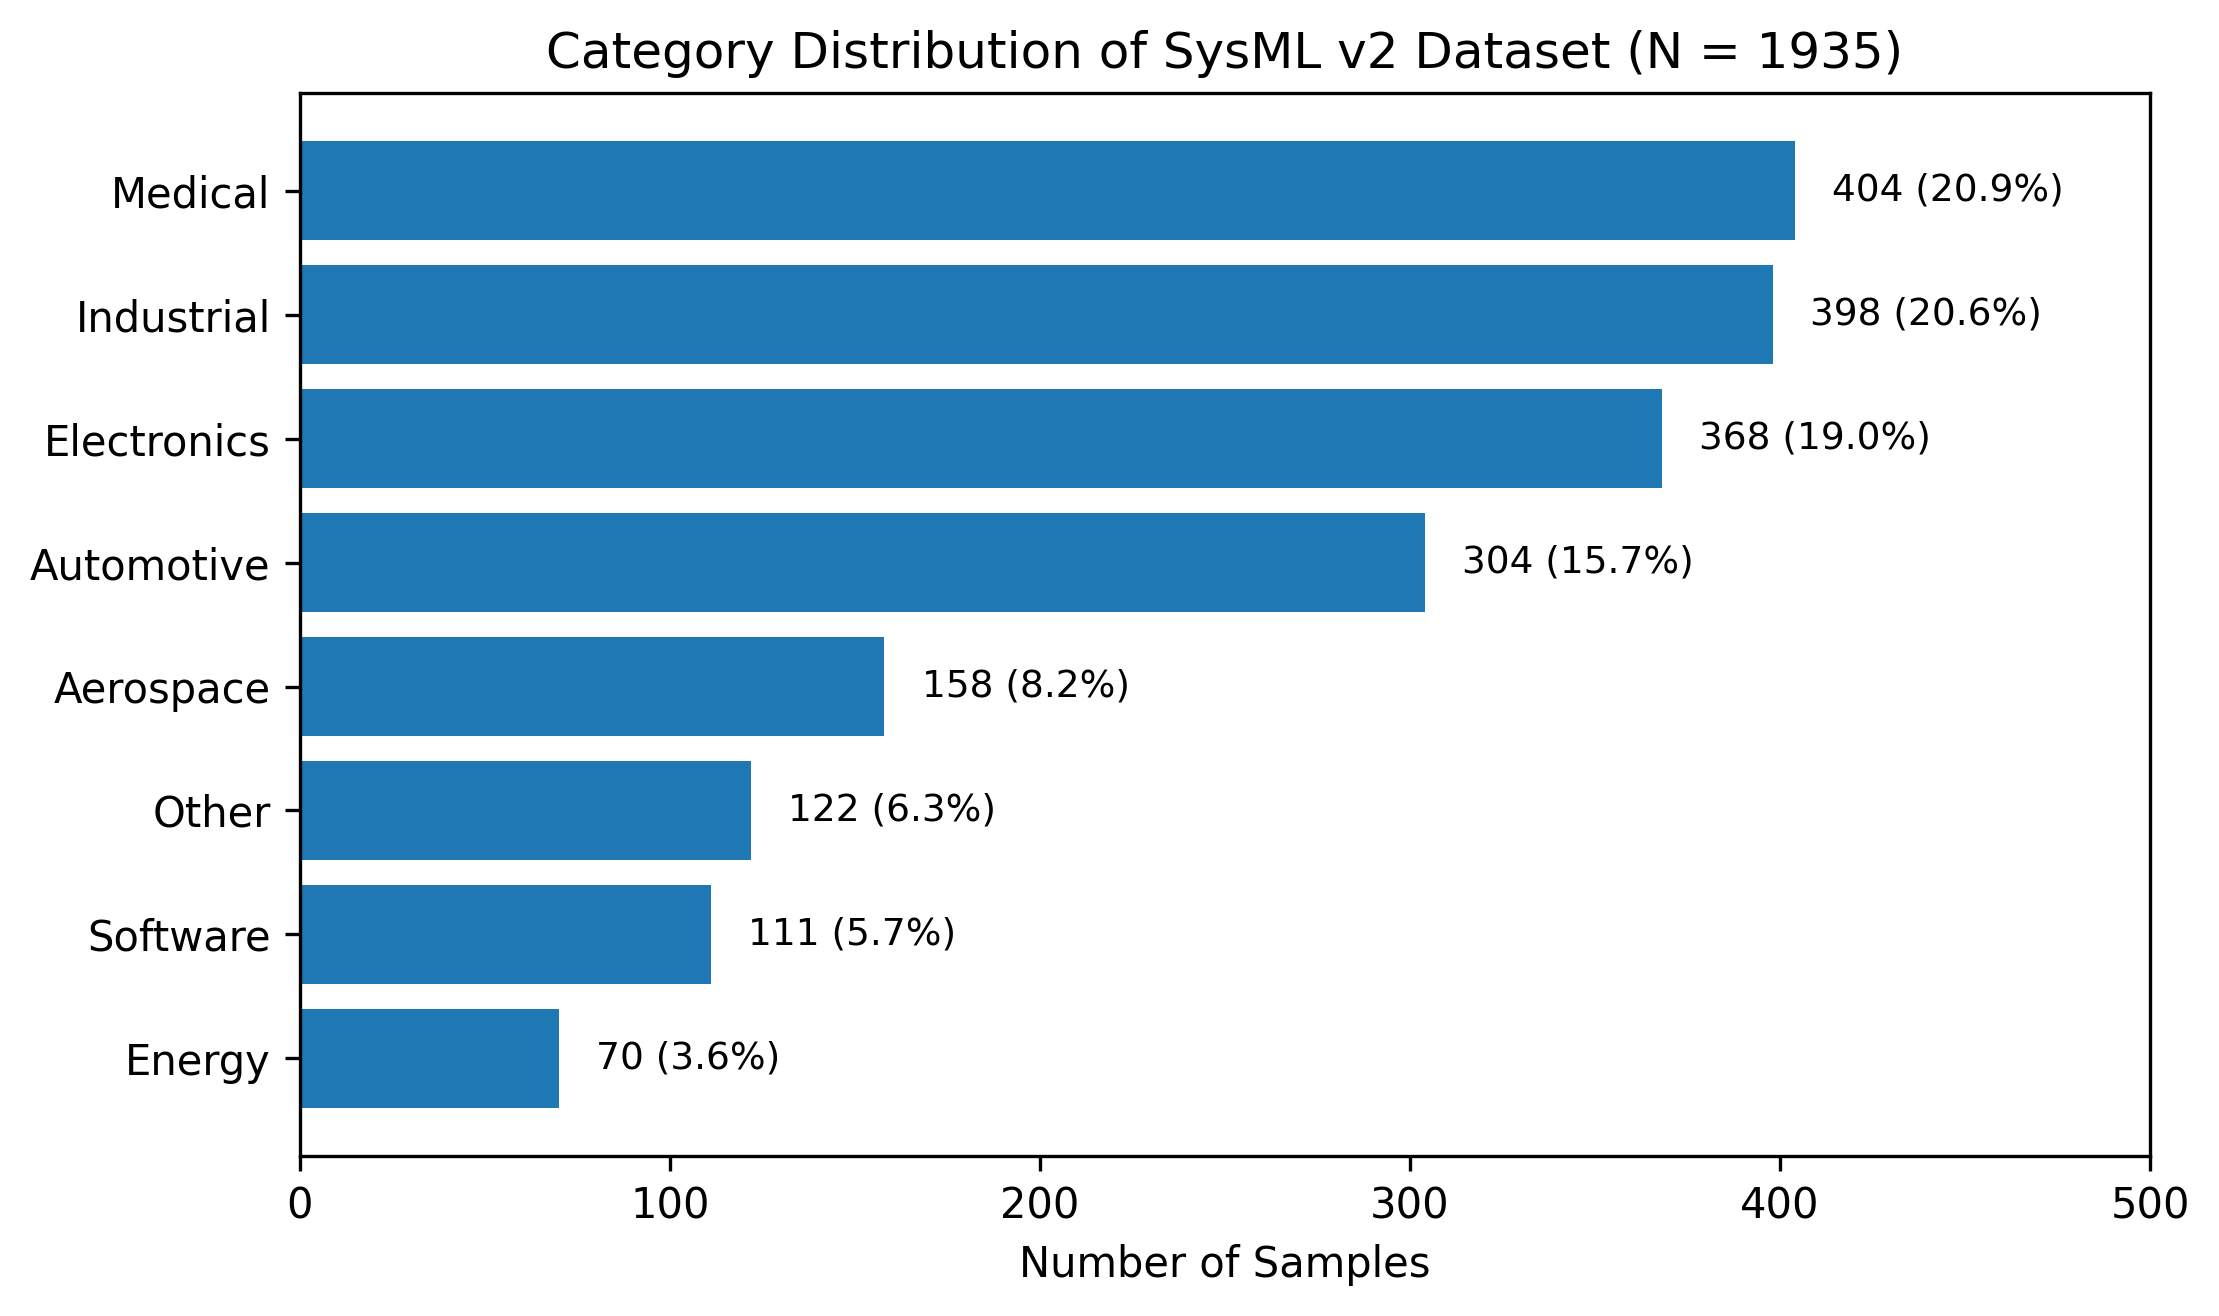
\includegraphics[width=\linewidth]{fig/sysml_v2_category_distribution.png}
  \caption{Category distribution of the SysML v2 dataset (N=1935), labeled by Gemini 2.5 Pro.}
  \label{fig:dataset-category}
\end{figure}

\begin{figure}[t]
  \centering
  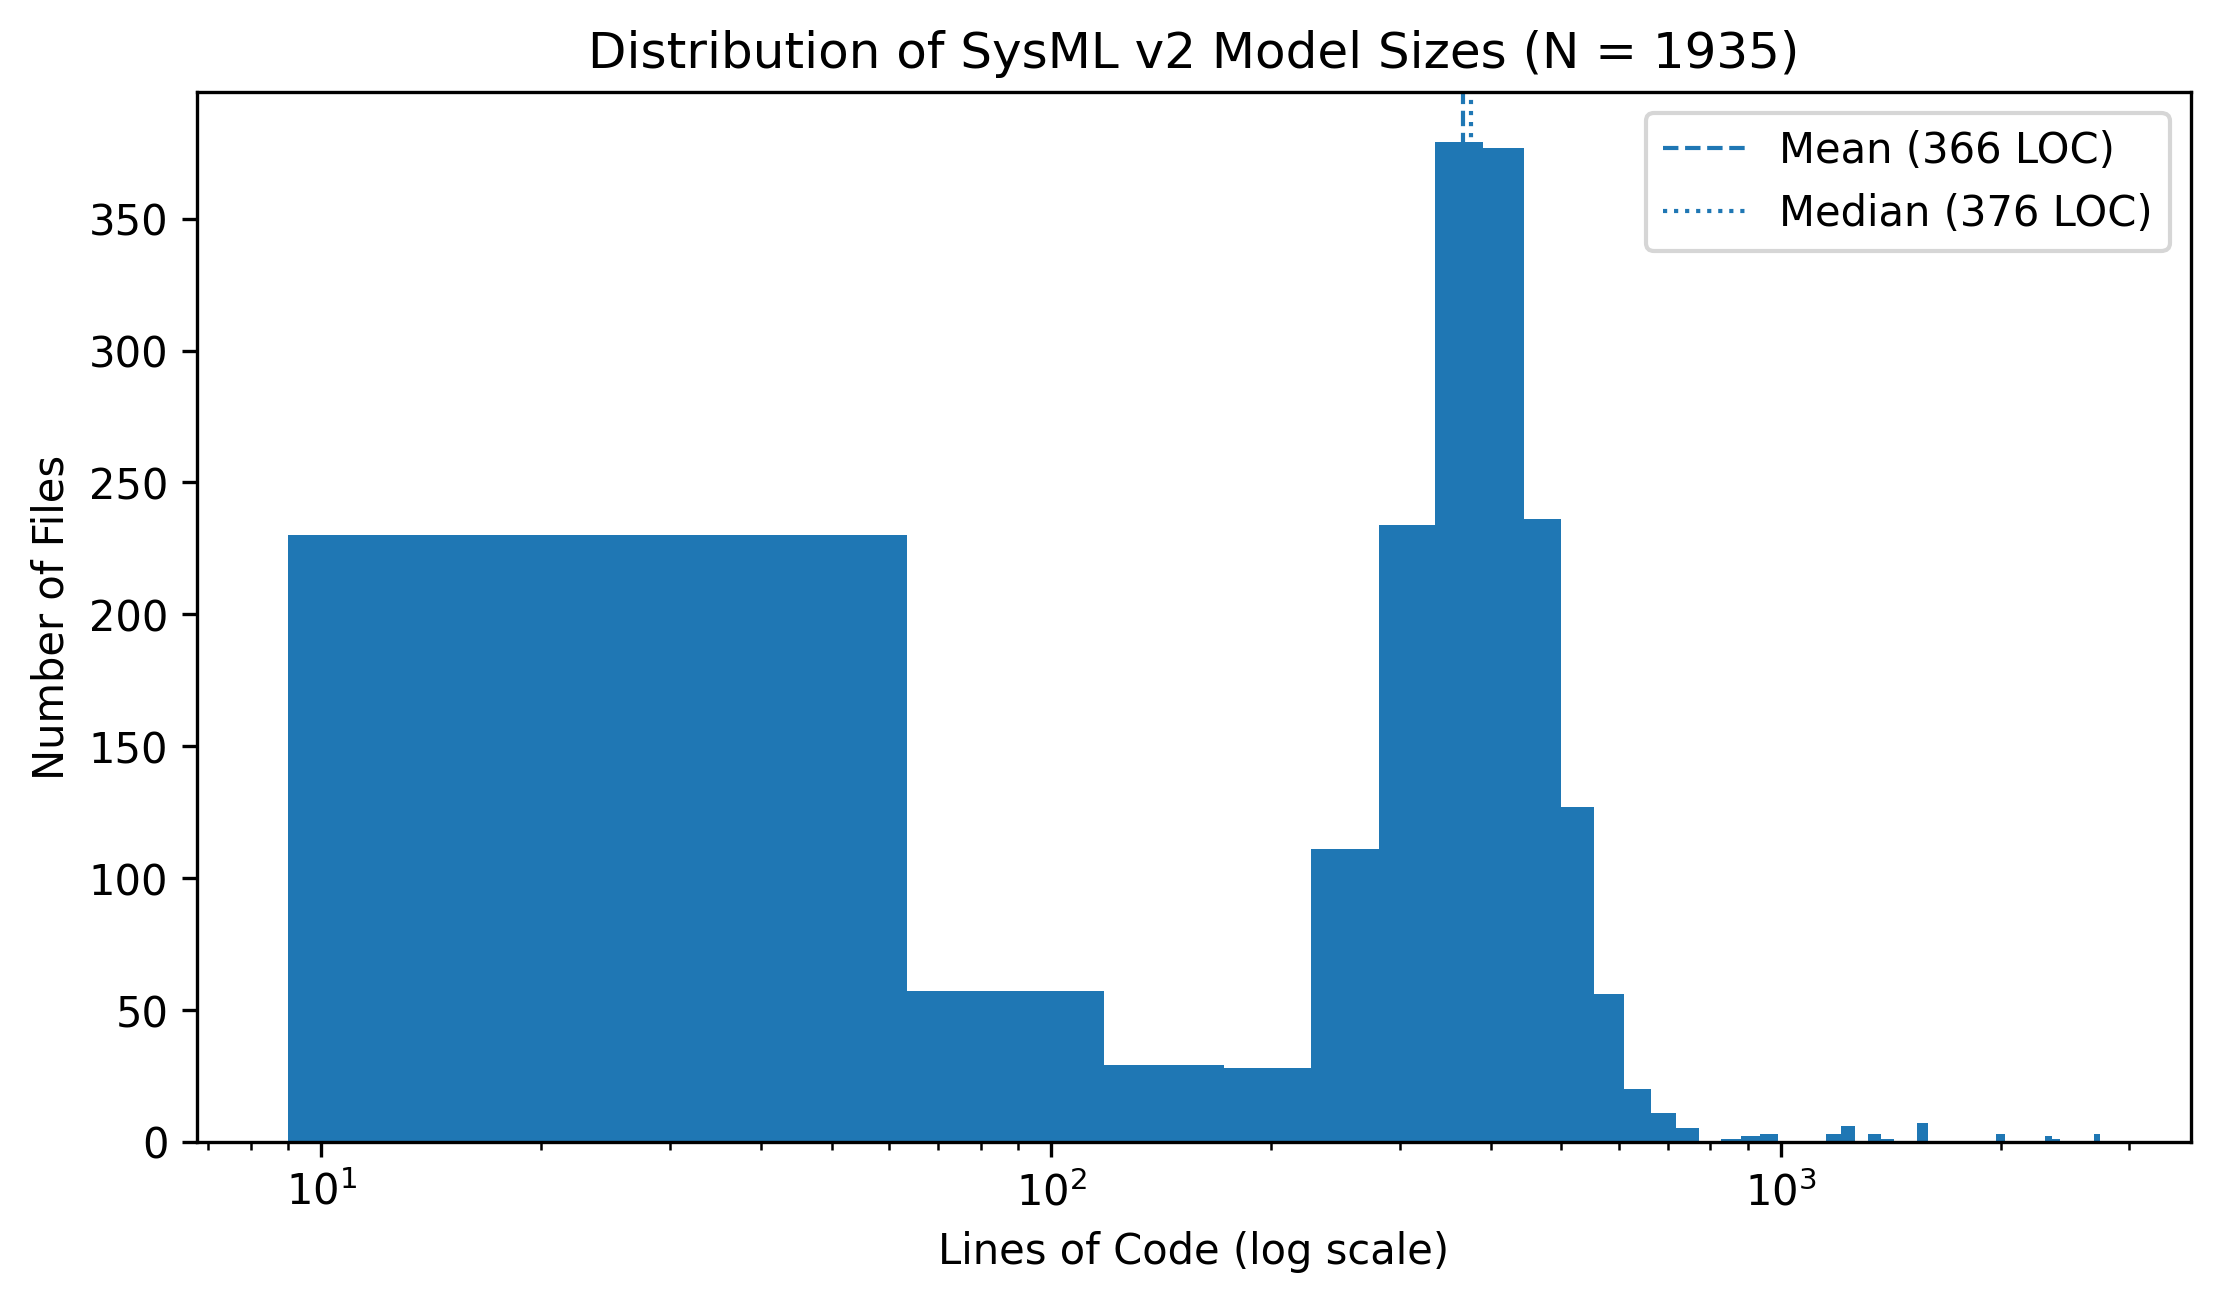
\includegraphics[width=\linewidth]{fig/sysml_v2_loc_distribution.png}
  \caption{Distribution of SysML v2 model sizes measured in lines of code (LOC), shown on a logarithmic x-axis (N=1935). Dashed and dotted lines indicate the mean (366 LOC) and median (376 LOC), respectively.}
  \label{fig:loc-distribution}
\end{figure}

Figure~\ref{fig:dataset-category} summarizes the category distribution of the SysML v2 dataset, where categories are labeled by Gemini 2.5 Pro. The dataset exhibits broad domain coverage, with a relatively balanced distribution across medical, industrial, and electronics systems, complemented by automotive and aerospace models, and smaller long-tail categories such as software and energy. Figure~\ref{fig:loc-distribution} characterizes model scale: sizes are well-centered around a few hundred LOC (mean 366; median 376), with a small number of substantially larger models forming a long tail on a logarithmic x-axis.

\subsection{Agent-Generated Data Quality}
We design the agent-generated subset to be both \emph{diverse} and \emph{reviewer-safe} for downstream modeling tasks. First, retrieval grounding anchors generation to in-domain exemplars and specification excerpts, reducing free-form drift. Second, MoE generation increases structural diversity while a combiner model consolidates candidates into a single coherent model. Third, we incorporate compiler feedback as a bounded repair loop and keep syntax-checked outputs whenever possible. Finally, we apply project-level splitting and structural-hash de-duplication (computed from canonicalized SysML2 text) to reduce leakage and near-duplicate inflation. We report per-source parse/compile success rates (Community/Wiki/Agent) after the full compilation pass.

\section{Experimental Evaluation}
\label{sec:experiments}

We structure the evaluation around five questions:
\begin{enumerate}
\item Evaluate current model ability on SysML embedding and retrieval.
\item Prove the agent generates good SysML v2 code.
\item Show performance across different data sources.
\item Compare model categories on the dataset.
\item Demonstrate that training on our dataset substantially improves performance.
\end{enumerate}

We follow a consistent retrieval protocol across experiments. For each split, queries are evaluated against the full candidate pool of that split (size: XX,XX). We use cosine similarity over $\ell_2$-normalized embeddings, with in-batch negatives and additional random negatives sampled from the same split; no cross-encoder re-ranking is applied. Reported metrics are averaged over both retrieval directions unless stated otherwise.

To ensure fair comparison across model classes, all embeddings are projected to a fixed dimension $d=\text{XX}$ and normalized before similarity. Encoder-only and encoder--decoder models use mean pooling over non-padding tokens; decoder-only models use last-layer mean pooling over non-padding tokens. Tokenization follows each model's native tokenizer, and all models are trained with the same batch size, temperature $\tau$, optimizer, and number of steps unless explicitly noted. For embedding-only baselines, the backbone is frozen unless the setting explicitly states fine-tuning.

\subsection{Embedding and Retrieval Ability}
This experiment establishes a zero-shot baseline for how well existing embedding models align SysML2 with natural language without any task-specific training. It answers whether the retrieval problem is already solvable with general-purpose embeddings and sets a reference point for subsequent improvements. We expect strong but uneven performance, with models trained on technical text performing better on Community and Wiki than on Migrate due to legacy syntax and longer sequences.
\begin{table}[H]
\centering
\small
\setlength{\tabcolsep}{3pt}
\caption{Zero-shot embedding baselines on SysML2--NL retrieval (R@5) by data source.}
\label{tab:sota-embeddings}
\begin{tabular}{lcccccc}
\toprule
Model & Off & Com & Pilot & ESA & Agent & All \\
\midrule
E5-large-v2 & XX.X & XX.X & XX.X & XX.X & XX.X & XX.X \\
GTE-large & XX.X & XX.X & XX.X & XX.X & XX.X & XX.X \\
Instructor-XL & XX.X & XX.X & XX.X & XX.X & XX.X & XX.X \\
BGE-large & XX.X & XX.X & XX.X & XX.X & XX.X & XX.X \\
\bottomrule
\end{tabular}
\end{table}

\subsection{Agent SysML v2 Code Generation}
Here we evaluate whether the agent can generate SysML v2 code that is not only textually similar to references but also syntactically valid and compilable. This is critical for practical deployment, since downstream tooling requires parseable models. We report exact match on canonicalized strings (comments and whitespace removed) and an element-level F1 computed over extracted SysML2 elements and relations. Parse/compile success are measured with the SysML v2 pilot parser and compiler (type resolution enabled); compile success requires all references to resolve. We expect the full agent (RAG + compiler feedback) to outperform ablated variants, with exact match remaining lower than structural metrics due to multiple valid encodings.
\begin{table}[H]
\centering
\setlength{\tabcolsep}{3pt}
\caption{SysML v2 generation quality for the agent; higher validity and exact match indicate better code synthesis.}
\label{tab:sysml-gen}
\begin{tabular}{lrrrr}
\toprule
Model & Exact & Elem-F1 & Parse & Compile \\
\midrule
Baseline & XX.X & XX.X & XX.X & XX.X \\
+RAG & XX.X & XX.X & XX.X & XX.X \\
+Feedback & XX.X & XX.X & XX.X & XX.X \\
\bottomrule
\end{tabular}
\end{table}
We also track compiler feedback cost, reporting the mean number of repair rounds per sample (XX.X) and the 95th percentile (XX.X).

\subsection{Source-wise Performance}
This experiment measures robustness across data sources and identifies domain shifts introduced by the collection pipeline. It is important for understanding whether models trained on mixed data generalize or disproportionately favor certain sources. We report after-training performance for the best model, and expect Wiki to show higher retrieval scores due to cleaner language, while Migrate likely lags because of converted syntax and longer structural dependencies.
\begin{table}[H]
\centering
\small
\caption{Retrieval performance by data source using the best trained model; source differences highlight domain shift.}
\label{tab:source-wise}
\begin{tabular}{lrrr}
\toprule
Source & R@1 & R@5 & MRR \\
\midrule
Community & XX.X & XX.X & XX.X \\
Wiki & XX.X & XX.X & XX.X \\
Migrate & XX.X & XX.X & XX.X \\
All & XX.X & XX.X & XX.X \\
\bottomrule
\end{tabular}
\end{table}

\subsection{Cross-Source Generalization}
We evaluate cross-source transfer by holding out one source at training time and testing on the held-out split. This highlights whether the embedding space captures structural alignment beyond source-specific distributions. We expect the largest degradation when holding out Migrate, reflecting the syntactic shift from converted v1 artifacts.
\begin{table}[H]
\centering
\small
\caption{Cross-source generalization with leave-one-source-out training (All metrics on the held-out source).}
\label{tab:cross-source}
\begin{tabular}{lrrr}
\toprule
Train Sources & Test Source & R@1 & MRR \\
\midrule
Community+Wiki & Migrate & XX.X & XX.X \\
Community+Migrate & Wiki & XX.X & XX.X \\
Wiki+Migrate & Community & XX.X & XX.X \\
\bottomrule
\end{tabular}
\end{table}

\subsection{Model Category Comparison}
We compare architectural families on a common dataset to assess which inductive biases are most suitable for joint embedding learning. This experiment motivates design choices for NExSys by isolating the effect of model class rather than training data. ``Before'' denotes pretrained models with the shared pooling and projection setup, without any task-specific fine-tuning; ``After'' denotes full joint training. We expect encoder--decoder models to achieve stronger retrieval due to richer cross-modal conditioning, while decoder-only models may lag on embedding quality but remain competitive when fine-tuned.
\begin{table}[H]
\centering
\small
\caption{Model class comparison on the full dataset; joint training yields consistent gains across architectures.}
\label{tab:model-class}
\begin{tabular}{lcrrr}
\toprule
Model Class & Training & R@1 & R@5 & MRR \\
\midrule
Embedding model & Before & XX.X & XX.X & XX.X \\
Embedding model & After & XX.X & XX.X & XX.X \\
Encoder-only & Before & XX.X & XX.X & XX.X \\
Encoder-only & After & XX.X & XX.X & XX.X \\
Encoder--Decoder & Before & XX.X & XX.X & XX.X \\
Encoder--Decoder & After & XX.X & XX.X & XX.X \\
Decoder-only & Before & XX.X & XX.X & XX.X \\
Decoder-only & After & XX.X & XX.X & XX.X \\
\bottomrule
\end{tabular}
\end{table}

\subsection{Effect of Training}
This experiment tests whether our dataset and training objective meaningfully improve retrieval performance over raw pretrained baselines. It directly validates the value of the curated pairs and the joint training objective. Hard negatives are constructed by selecting nearest-neighbor SysML2 fragments from the same domain but with different element identifiers and requirements; these are mixed with random in-batch negatives. We anticipate the largest gains on hard negatives, since training explicitly introduces structured negatives and forces models to discriminate semantically close SysML2 fragments.
\begin{table}[H]
\centering
\small
\caption{Task-wise retrieval on the full dataset; hard negatives remain the most challenging setting despite training.}
\label{tab:task-wise}
\begin{tabular}{llrrr}
\toprule
Task & Model & R@1 & R@5 & MRR \\
\midrule
\multirow{3}{*}{NL $\rightarrow$ SysML} & Embedding & XX.X & XX.X & XX.X \\
 & Encoder--decoder & XX.X & XX.X & XX.X \\
 & Decoder-only & XX.X & XX.X & XX.X \\
\midrule
\multirow{3}{*}{SysML $\rightarrow$ NL} & Embedding & XX.X & XX.X & XX.X \\
 & Encoder--decoder & XX.X & XX.X & XX.X \\
 & Decoder-only & XX.X & XX.X & XX.X \\
\midrule
\multirow{3}{*}{Hard Negative} & Embedding & XX.X & XX.X & XX.X \\
 & Encoder--decoder & XX.X & XX.X & XX.X \\
 & Decoder-only & XX.X & XX.X & XX.X \\
\bottomrule
\end{tabular}
\end{table}

We also evaluate robustness to non-semantic perturbations that should preserve meaning, including alpha-renaming of identifiers, statement reordering, and formatting changes. This tests whether models are sensitive to surface forms rather than SysML2 structure.
\begin{table}[H]
\centering
\small
\setlength{\tabcolsep}{3pt}
\caption{Robustness to non-semantic perturbations; higher scores indicate invariance to surface changes.}
\label{tab:robustness}
\begin{tabular}{lrrr}
\toprule
Perturbation & Embedding & Enc--Dec & Dec-only \\
\midrule
Alpha-renaming & XX.X & XX.X & XX.X \\
Reordering & XX.X & XX.X & XX.X \\
Formatting & XX.X & XX.X & XX.X \\
\bottomrule
\end{tabular}
\end{table}

\section{Analysis and Discussion}
\label{sec:analysis}

% PLACEHOLDER: Analysis section covering:
% - NExSys embedding space visualization (t-SNE, UMAP)
% - Semantic similarity analysis
% - Cross-domain transfer capabilities of NExSys
% - Error analysis and failure modes
% - Computational efficiency analysis of NExSys variants
% - Limitations and edge cases

\section{Conclusion}
\label{sec:conclusion}

We have presented NExSys (\textbf{N}aturally \textbf{Ex}pressive \textbf{Sys}tems Engineering), a novel framework for learning joint embeddings between natural language and SysML2 through contrastive learning with the Qwen model family. NExSys represents the first large-scale effort to bridge the semantic gap between informal natural language descriptions and formal systems modeling specifications using modern deep learning techniques.

The key insights from NExSys are threefold. First, contrastive learning provides a natural framework for capturing the semantic correspondence fundamental to requirements traceability in systems engineering. By learning to align natural language and SysML2 representations in a shared embedding space, NExSys enables a range of downstream applications from automated documentation to semantic search. Second, the hierarchical nature of systems models demands hierarchical learning objectives—NExSys's multi-granularity contrastive losses significantly outperform flat approaches by respecting the compositional structure of both modalities. Third, the choice between NExSys-Encoder and NExSys-ED architectures should be task-dependent: encoder-only models excel at embedding-based retrieval and similarity tasks, while encoder-decoder variants prove superior for generation tasks requiring sequential output.

Our empirical results demonstrate state-of-the-art performance across multiple evaluation tasks. On SysML2-to-text generation, NExSys-ED achieves XX.X BLEU score, substantially outperforming baseline approaches. For the inverse task of text-to-SysML2 synthesis, NExSys-ED achieves XX\% exact match accuracy on held-out test examples. Cross-modal retrieval experiments using NExSys-Encoder show Recall@10 of XX.X\%, enabling practical semantic search applications. Requirements traceability tasks, evaluated on industrial case studies, demonstrate XX.X\% precision and XX.X\% recall in identifying correspondence between informal requirements and formal model elements using NExSys embeddings.

Beyond quantitative metrics, our analysis reveals several important findings about the NExSys embedding space. Visualization studies show clear semantic clustering by domain (aerospace, automotive, robotics) and abstraction level (requirements, components, behaviors). Cross-domain transfer experiments indicate that NExSys models trained on diverse domains generalize better to new domains than domain-specific models, suggesting that NExSys learns domain-agnostic principles of language-model correspondence. Error analysis identifies several challenging cases including highly technical domain-specific terminology, complex nested hierarchies, and implicit semantic relationships—these cases motivate future research directions for enhancing NExSys.

The implications of NExSys for systems engineering practice are significant. NExSys enables AI-assisted workflows that reduce the manual effort in requirements engineering, improve consistency between informal and formal artifacts, and make complex models accessible to stakeholders without modeling expertise. Early adoption in industrial partners indicates potential productivity improvements of XX-XX\% in requirements formalization tasks using NExSys, though comprehensive longitudinal studies are needed to validate these preliminary findings.

\textbf{Future Directions:} Several promising directions emerge from the NExSys framework. First, incorporating structural inductive biases specific to SysML2's metamodel (typing relationships, specialization hierarchies, conjugation semantics) could improve NExSys representation quality beyond purely sequence-based modeling. Second, active learning approaches could identify high-value examples for annotation, addressing the data collection bottleneck for expanding NExSys training data. Third, integrating formal verification and model checking into the NExSys training loop could enforce semantic validity beyond syntactic correctness. Fourth, extending NExSys to other systems engineering artifacts (test cases, simulation configurations, interface specifications) could provide a more comprehensive MBSE automation framework. Finally, investigating few-shot and zero-shot transfer of NExSys to specialized domains (medical devices, avionics, energy systems) would assess the practical applicability across the full spectrum of systems engineering domains.

We release our curated dataset, NExSys model checkpoints, and evaluation code to support reproducibility and encourage further research at the intersection of natural language processing and model-based systems engineering.

\section*{Acknowledgments}

% PLACEHOLDER: Add acknowledgments

\bibliography{references}
\bibliographystyle{icml2026}

% PLACEHOLDER: Create separate references.bib file with complete citations

\appendix

\section{Appendix}
\label{sec:appendix}

% PLACEHOLDER: Appendices for:
% - Additional NExSys experimental results
% - Dataset examples and statistics
% - NExSys hyperparameter sensitivity analysis
% - Qualitative examples and case studies
% - Computational cost breakdown for NExSys variants
% - Ethical considerations for NExSys deployment
% - NExSys model architecture diagrams
% - Complete ablation study results

\end{document}
